\chapter{Introduction to Ginan GNSS Processing Toolkit}
\label{ch:introduction}

Ginan\footnote{\url{https://github.com/GeoscienceAustralia/ginan}} is a collection of source code that is currently made up two distinct software repositories, the POD and the PEA.
Using the POD and PEA together will allow you to estimate your own satellite orbits from a global tracking network.
The POD (precise orbit determination) contains all of the source code needed to determine a GNSS satellite's orbit. You can establish the initial conditions of an orbit from a broadcast ephemeris file, or from an IGS SP3 file. It can then estimate it's own orbital trajectory based upon the models specified in configuration files, and output an SP3 file, or provide a partial files which can then be updated from a tracking network. 


The PEA (parameter estimation algorithm) takes raw observations in RINEX format or in RTCM format, to estimates the parameters you are interested in. You can run it a single user mode, taking in orbit and clocks supplied by real-time streams to SP3 files obtained from the IGS to estimate your own position in static and kinematic mode. 
You can also run the PEA in a network mode, and take in a global network of observations to determine your own orbits and satellite clocks to support your application.

\begin{figure}
	\centering
	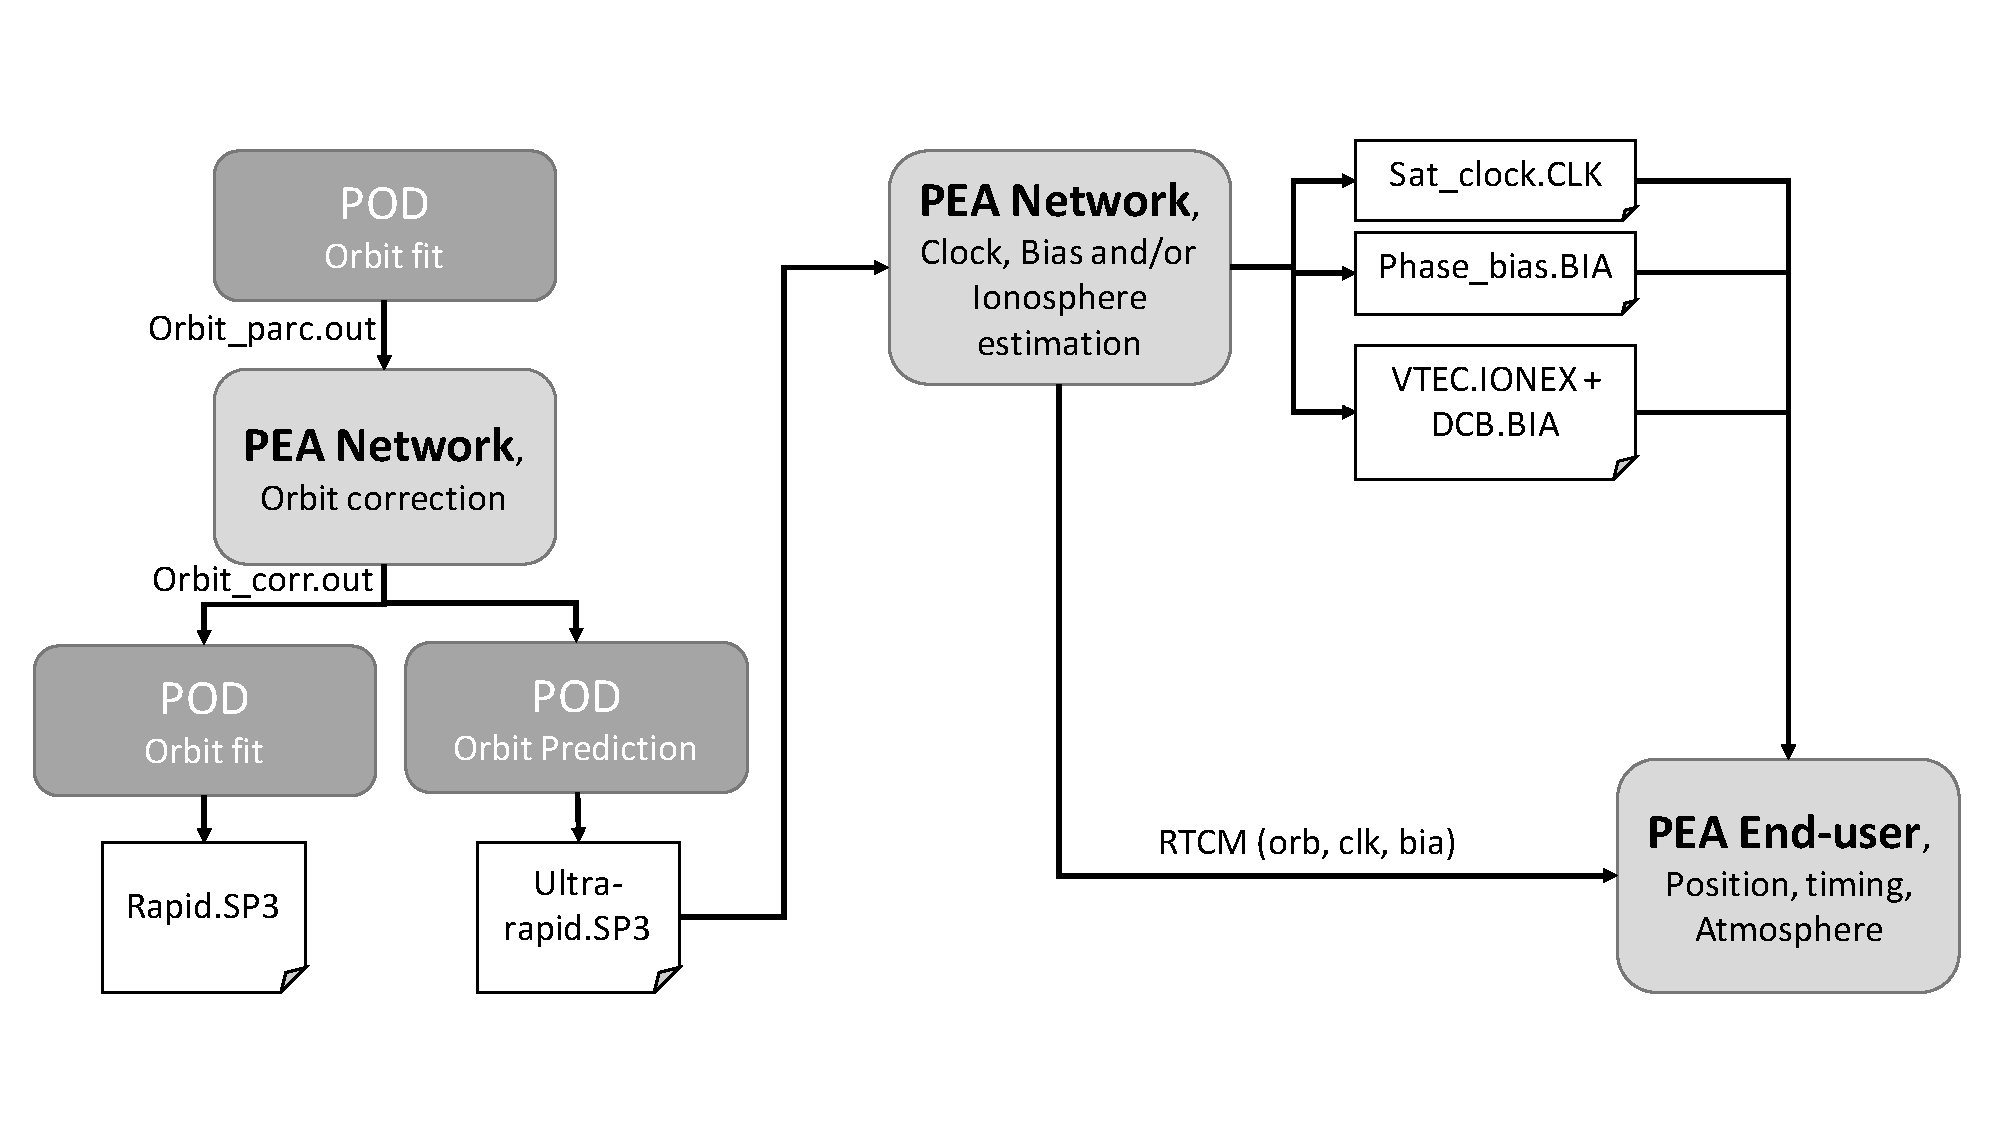
\includegraphics[width=\linewidth]{Figures/Ginan_diagram.pdf}
	\caption{Ginan software components}
	\label{fig:PEAnPOD}
\end{figure}

The software is aimed at supporting Australia's implementation of a national positioning infrastructure that supports the objective of 'instantaneous GNSS positoning anywhere, anytime, with the highest possible accuracy and the highest possible integrity.

\textbf{Carrier phase ambiguity}. The underlying signals transmitted by the Global Navigation Satellite Systems (GNSS) can be considered as waves, just like repeating sine waves from high school mathematics. Measurements of these waves are referred to as carrier phase observations, and they are used to provide the precise distance, with mm precision and accuracy, between the orbiting satellites and user’s receiver that are subsequently used to compute position. However, a complicating factor is that carrier phase observations have an ambiguous component where the total whole number of waves, or integer cycles, between the satellite and the user’s receiver cannot be measured, only the fractional part. The unknown number of integer cycles is called the carrier phase ambiguity. Fortunately, the ambiguities can be estimated, and the mathematical and statistical solution to this problem is known as integer ambiguity estimation. While there is a long history of research in this area, which has largely focused on GPS applications, the most optimal solution to this problem when simultaneously combining data from all the GNSS remains unresolved.

\textbf{Atmosphere delay of GNSS signals}. The Earth is surrounded by layers of gases held by Earth's gravity. Signals, such as those transmitted by GNSS, propagated from space are delayed as they pass through the atmosphere. In the troposphere, the region from the Earth’s surface to approximately 20 km altitude, the delay is proportional to temperature, pressure and humidity. The ionosphere, the region from 50-1000 km altitude, causes delay as a function of the frequency of the signal. The composition of both the troposphere and ionosphere vary both in space and time, and this variability currently limits the accuracy, speed and reliability of positioning. But it’s not all bad news, and like a CAT scan in medical science, the new GNSS signals and satellites can potentially be combined to provide a more complete three dimensional picture of the atmospheric delay as a function of time. Models that more completely remove the nuisance atmospheric signals will lead to improved accuracy, speed and reliability of positioning.

\textbf{Precise Point Positioning (PPP) and Real Time Kinematic (RTK)}. Conventional positioning technologies almost exclusively use a technique called Real Time Kinematic (RTK). The RTK technique takes information from nearby Continuously Operating Reference Stations (CORS) to generate corrections for measurements made by users. One of the most important of these is the carrier phase ambiguity correction. The ability to correctly determine carrier phase ambiguities with RTK is determined by many factors, such as the distance between the reference stations and the user and also atmospheric effects. Consequently, RTK relies on relatively dense CORS networks with a typical spacing of 30 to 70 km. An alternative to RTK is Precise Point Positioning (PPP). The PPP technique, rather than directly using measurements from nearby reference stations, uses global satellite orbit and clock information such as that provided by the International GNSS Service. The major advantage of PPP is that it doesn’t require a dense CORS network nearby the user’s location just access to global products. Unfortunately, the PPP technique can have difficulties in resolving carrier phase ambiguities in real time, but additional research focused on greater exploitation of multi-GNSS data and more regional approaches may in the future overcome this limitation.